\chapter{Excitación de iones por impacto de electrones}

%=======================================================================
\section{Introducción}
\label{sec:intro}

El espectro de átomos complejos en diversos estados de ionización son 
emitidos por objetos astronómicos, la corona solar, nebulosas, quasars, 
etc, y también en descargas en laboratorios terrestres. La interpretación
de dichas observaciones requiere de una extensa variedad de datos 
atómicos. Los cálculos de niveles de energía son utilizados como una guía
para identificar las líneas espectrales observadas , mientras que sus 
intensidades requieren la determinación de secciones eficaces 
colisionales y fuerzas de oscilador.

La teoría de la estructura atómica se describe en el trabajo fundamental
de Condon y Shortley (1935). La teoría de átomos complejos altamente 
ionizados fue extendida por Layzer (1959), quien mostró que, como 
consecuencia de la degeneración del momento angular $l$ en el límite 
hidrogénico, es necesario introducir la interacción de todas las 
configuraciones que cuenten con la misma paridad y el mismo conjunto de 
números cuánticos principales.

La descripción precisa de la excitación por impacto de electrones de los 
iones atómicos sigue siendo una de las tareas más desafiantes para los 
métodos avanzados, tales como el acoplamiento cercano convergente 
(convergent close--coupling, CCC)~\cite{Bray:92}, el acoplamiento cercano 
de matriz R (R-matrix close--coupling)~\cite{Burke:75} y el acoplamiento 
cercano dependiente del tiempo (time--dependent close--coupling) 
\cite{Pindzola:07}, aún en las máquinas con enorme poder computacional.
%En el caso de los sistemas ``simples'', esta complejidad puede deberse al 
%requisito de una descripción completa de todos los parámetros de 
%dispersión o simplemente a las secciones transversales totales en el caso 
%de estados muy excitados. Para los sistemas ``complejos'', la cantidad de 
%canales de dispersión en sí mismos puede ser abrumadora. 
El modelado de diagnóstico espectroscópico de plasmas astrofísicos y de 
laboratorio tiene un gran apetito por los coeficientes de tasa de 
excitación de impacto de electrones, ya que determinan en gran medida la 
distribución de la población emisora dentro de un estado de carga. El 
método de acoplamiento cercano puede, en principio, proporcionar datos 
de excitación entre todos los estados objetivo incluidos en su expansión.



\begin{comment}
La importancia de la correcta representación de la estructura atómica al 
describir la excitación por impacto de electrones ha sido estudiada y 
demostrada usando diversos métodos no perturbativos de acoplamiento 
cercano (close--coupling, CC) \cite{Bartschat:04,Zatsarinny:16,
Be_Ballance:03} para un gran número de blancos. Particularmente, en 
blancos neutros y de bajo grado de ionización, existe un gran número de 
trabajos de investigación~\cite{Ballance:03,Badnell:03,Mitnik:03} que han 
demostrado la importancia del acoplamiento al continuo del blanco para 
describir correctamente este proceso. Sin embargo, la determinación de 
una adecuada representación del blanco no es condición suficiente. La 
apropiada resolución del problema colisional requiere además un amplio 
conocimiento sobre el método y, en general, grandes recursos 
computacionales.

De Bautista (2008)

Various methods are known that allow one to model the structure of atoms 
and ions, such as Hartree-Fock, multiconfiguration Hartree-Fock,
superposition of configurations, semi-empirical methods, many-body 
perturbation methods and central field approximation methods, etc. 
Methods based on the Hartree-Fock formalism are self-consistent and can 
yield very accurate results for simple atoms or for a few select levels 
of more complex systems. Methods based on the central field approximation 
that allow for configuration interaction have been successful in 
describing large numbers of levels for more complex systems, such as 
metals. However, computations of large scale models of 3d transition 
metals remain quite challenging. In order to obtain accurate (∼10%) 
radiative rates and cross sections for photon and electron interactions 
one needs to guarantee eigenenergies that compare well (within ∼5%) with
experimentally determined energies. However, this is difficult to achieve 
with ab initio calculations for ions with more than just a few electrons. 
Moreover, comparisons are regularly done with energies relative to the 
ground level, which can be misleading if the absolute energy of the 
ground level is overestimated. 

An approach sometimes used in complex systems to include missing 
core-valence correlations is the use of ad hoc polarization model 
potentials~ \cite{Norcross:76}. These model potentials work well for 
alkalies with a single electron outside the core. For systems with two 
valence electrons polarization model potentials can also be constructed
by including dipole and quadrupole polarizations. However, for systems 
with more than two electrons outside the core, such as transition metals 
with several 3d electrons, polarization model potentials are generally 
inapplicable. This is because: (1) one cannot define a closed 3p6 core 
due to the strong 3p-3d correlations, and (2) treatment of multiple 
electrons outside the core requires several high-order correction terms 
beyond the dipole one that make such models impractical.

\end{comment}

\newpage
%=======================================================================
\section{Descripción del blanco}

En general, la función de onda de los blancos atómicos se expresa 
implementando el método de interacción de configuraciones (configuration
interaction, CI); esto es,
\begin{equation*}
\Psi_i(\mathbf{r}) =
\sum_j^{N} c_{ji} \, \Phi_j(\mathbf{r})\,,
\end{equation*}
donde $N$ es el número de configuraciones electrónicas relevantes dentro
de la aproximación de interacción de configuraciones, y $\Phi_j$ son las
funciones de onda correspondientes a cada configuración. Dentro de la 
aproximación de electrón activo, la parte radial de las funciones de 
onda electrónicas se obtienen a partir de la resolución de la ecuación 
de Schr\"odinger radial de un electrón,
\begin{equation*}
\left[ \frac{1}{2} \frac{d^2}{dr^2} - \frac{l(l+1)}{2r^2} 
 + V_j^{\mbox{\scriptsize eff}}(\lambda_j,r)
 + E_j \right] P_j(r)=0\,,
\end{equation*}
donde $V_j^{\mbox{\scriptsize eff}}$ es un potencial modelo, que puede 
ser ajustado a partir de un parámetro de escala 
$\boldsymbol\lambda=\{\lambda_j\}$. 


\subsection{Potenciales modelo}

Existen diversos potenciales modelos que permiten el cálculo de la
estructura del blanco. En esta sección, nos centraremos en dos de los más 
usados: el potencial de Thomas-Fermi-Dirac-Amaldi (TFDA) y el potencial 
de orbitales tipo Slater (STO) de Burgess.

\subsubsection*{Potencial TFDA}

El potencial de Thomas-Fermi~\cite{Gombas:56,Eissner:69,Bautista:08} para 
una carga electrónica a una distancia $r$ del núcleo está dada por
\begin{equation}
V(r)=-\frac{2Z}{r}+\int_0^{r_0}\frac{2}{r_>} \rho(r')4\pi r'^2\,dr'\,,
\label{eq:Thomas-Fermi}
\end{equation}
donde $\rho(r)$ es la densidad de carga, $r_>$ es el mayor valor de entre
$r$ y $r'$, y $r_0$ es el radio de la superficie del átomo. El último
término del lado derecho surge de la aproximación clásica para una 
densidad de carga esféricamente simétrica. 

La energía total de este átomo está dada por la suma de sus valores 
cinéticos y potenciales; esto es,
\begin{equation}
E=\int_0^{r_0}\left[\frac{3}{5}(3\pi^2)^{2/3}\rho^{2/3}(r)-\frac{2Z}{r}
+\frac{1}{2}\int_0^{r_0}\frac{2}{r_>}\rho(r')4\pi r'^2\,dr'\right] 
\rho(r)4\pi r^2\,dr\,.
\label{eq:tot-ener-TF}
\end{equation}
Para valores de radio tal que $r\leq r_0$, la expresión de $E$ es 
minimizada para un valor de $\rho$ que satisface la relación
\begin{equation}
\left[3\pi^2\rho(r)\right]^{2/3}+V(r)-V_0=0\,, 
\end{equation}
donde, para un átomo aislado, la densidad electrónica debe ser cero en
$r=r_0$, y 
\begin{equation}
V_0=V(r_0)=-\frac{2(Z-N)}{r_0}
\end{equation}

Sin embargo, el modelo de Thomas-Fermi sólo contempla interacciones 
electrostáticas núcleo-electrón y electrón-electrón. Los efectos de 
intercambio electrónico fueron introducidos por Dirac. Sin embargo, la 
acción sobre cada electrón en este modelo está determinada por el campo 
resultante de los $N$ electrones; esto conduce al famoso problema de la 
auto-interacción de los electrones. Amaldi y Fermi corrigieron este 
inconveniente, y, ahora la ecuación (\ref{eq:tot-ener-TF}) es minimizada
para una de densidad de carga que está dada por
\begin{equation}
\rho(r)=\frac{1}{2\pi^2}\left\{\frac{1}{\pi}+\left[\frac{1}{\pi^2}+V_0-
V(r)\right]^{1/2}\right\}^3\,,
\end{equation}
y
\begin{equation}
V_0=-\frac{15}{16\pi^2}-\frac{2(Z-N)}{r_0}\,.
\end{equation}
Finalmente, se introduce un factor de escala en el potencial, tal que
\begin{equation*}
 V^{\textrm{TFDA}}(\lambda_i,r) = V(r/\lambda_i)\,.
\label{eq:TFDA-pot}
\end{equation*}

\subsubsection*{Potencial STO}

En el esquema del potencial de Burgess~\cite{Burgess:89}, se asume que 
cada uno de los electrones ligados se mueve en un potencial apantallado 
independiente, que es generado por una carga nuclear $Z$ y la 
distribución de carga de los $N-1$ electrones restantes. Se implementan 
orbitales de tipo Slater (Slater-type orbitals, STO) $p_j(r)$ para 
calcular la contribución a esta distribución de carga por parte de los 
$q_j$ electrones en la $j$-ésima subcapa $n_jl_j$. Estos orbitales están 
dados por
\begin{equation}
p_j(r) = c\rho_j^n e^{-\rho_j/2}\,,
\end{equation}
donde $c$ es una constante de normalización, y 
\begin{equation}
\rho_j= \frac{2z_j\lambda_jr}{n_j}\,
\end{equation}
donde $\lambda_j$ es un parámetro de escala y 
\begin{equation}
z_j=Z-\frac{1}{2}\left(q_j-1\right)-\sum_{i<j} q_s\,.
\end{equation}
A una distancia $r$ del núcleo, cada uno de estos electrones genera un 
apantallamiento 
\begin{equation}
\frac{\left[\int_0^r p_j(\xi)\,d\xi +r\int_r^{\infty}
\frac{p_j(\xi)}{\xi}\,d\xi\right]}{\int_0^{\infty}p_j^2(\xi)\,d\xi}\,.
\end{equation}
Así, el potencial al que está sujeto un electrón fuera el la subcapa 
$i$-ésima es
\begin{equation}
V_i^{\textrm{STO}}(r)=-\frac{1}{r}\left\{Z-\sum_j(q_j-\delta_{ij})\left[1-
\frac{e^{-\rho_j}}{2n_j}\sum_{m=0}^{2n_j-1}\frac{(2n_j-m)}{m!}\rho_j^m
\right]\right\}\,.
\label{eq:STO-pot}
\end{equation}

\subsection{Potenciales de polarización}

En sistemas con ``núcleos electrónicos'' o \textit{cores} polarizables y 
pocos electrones de valencia, los efectos de correlación suelen ser 
significativos y deben ser considerados. En general, estos efectos son 
pronunciados en átomos alcalinos y alcalinotérreos, incrementando sus 
energías de ionización, contrayendo su capa de valencia, reduciendo 
polarizabilidades y fuerzas de oscilador~\cite{Muller:83}. 
Así, para obtener una representación precisa de las funciones de onda de 
átomos alcalinos y alcalinotérreos, es importante considerar no sólo las 
correlaciones de valencia, sino también las core-valencia 
\cite{Bartschat:04}. Una posible forma de incluir los efectos de 
correlación core-valencia está dado por la inclusión de potenciales de 
polarización de core semi-empíricos~\cite{Loughlin:88}.

\begin{comment} (sigue de Bartschat)
Although such a potential simplifies the calculations significantly and 
may yield accurate excitation energies and oscillator strengths, the 
question always remains how well the model potential can really simulate 
all core–valence correlation effects, including non-dipole contributions.
\end{comment}
Existen diversas aproximaciones de los efectos de correlación de los 
electrones pertenecientes a las capas más internas y los electrones de 
valencia~\cite{Seaton:72,Loughlin:73,Migdalek:78}. En este trabajo, 
incluimos estos efectos a partir del potencial de polarización de 
Norcross~\cite{Norcross:76}. Este potencial modelo está basado en un 
Hamiltoniano de dos electrones y un modelo de \textit{frozen-core} en 
Be I.
\begin{equation*}
 V_{\textrm{pol}}(r) = -\frac{\alpha_l}{r^4}\left[1-
e^{-\left(\tfrac{r}{\rho_l}\right)^6}\right]
\label{eq:Norcross-pot}
\end{equation*}

\subsection{Pseudo-orbitales}

Los pseudo-orbitales se escriben en términos de funciones de onda 
radiales de Laguerre no-ortogonales de la forma
\begin{equation}
P_{nl}(r) = N_{nl}(\lambda_{nl}Zr)^{l+1} e^{-\lambda_{nl}Zr/2} 
L_{n+l}^{2l+1}(\lambda_{nl}Zr)\,.
\label{eq:pseudo}
\end{equation}

La precisión de los cálculos de estructura del blanco aumenta con el 
número de 
configuraciones en el CI, lo que en efecto incrementa el número de 
parámetros que definen el problema. Sin embargo, no existe aún un método 
sistemático que permita encarar exitosamente la optimización.



\newpage
\subsection{Ejemplo: influencia de la descripción blanco}
%%%%%%%%%%%%%%%%%%%%%%%%%%%%%%%%%%%%%%%%%%%%%%%%%%%%%%%%%%%%%%%%%%%%%%%%%
\begin{figure}[t]
\centering
\includegraphics[width=\textwidth]{figures/rmatrix/example_PS.eps}
\caption[Dependencia de la sección eficaz de excitación con las 
configuraciones electrónicas y los pseudoestados.]
{Dependencia de la sección eficaz de excitación por impacto de
electrón con las configuraciones electrónicas incluidas en el CI 
(izquierda) y los pseudoestados (derecha) para la transición dipolar 
prohibida $2s^2\,^1S \rightarrow 2s3s\,^1S$ de Be.}
\label{fig:dependencia-CI}
\end{figure}

La dependencia de las secciones eficaces de excitación por impacto de 
electrón con las configuraciones incluídas en el CI se ilustra en el 
panel izquierdo de la figura~\ref{fig:dependencia-CI} para la transición 
$2s^2\,^1S\rightarrow 2s3s\,^1S$ del átomo de berilio. Las curvas 
muestran los resultados de los cálculos colisionales con el método de 
R-Matrix cuando se han definido 6 (línea de puntos), 13 (línea 
punto-raya) y 27 (línea discontinua corta) configuraciones electrónicas 
en la mezcla. En el primer caso, se han incluido las configuraciones 
$2s^2$, $2snl$ con $n=1-3,l=0-2$ y $2p^2$. En el segundo, además se han 
incorporado las configuraciones $2snl$ tal que $n=4,l=3$. Mientras que en 
el último caso, también se han incluido las excitaciones de un electrón a 
los términos con números cuánticos $n=5,l=4$. Por otro lado, el panel 
derecho de la figura~\ref{fig:dependencia-CI} muestra las secciones 
eficaces para la misma transición en Be, pero ahora se ha reemplazado un 
conjunto de orbitales espectroscópicos por pseudo-orbitales. En la parte 
superior de ambos paneles se ilustran las energías de todos los términos 
incluidos en cada cálculo. En este caso, no hemos realizado 
optimizaciones en el blanco (variación de parámetros). Así, sólo se 
observan los efectos de la inclusión de nuevas configuraciones 
electrónicas en el CI y de pseudo-orbitales. En el panel izquierdo, 
notamos como para esta transición dipolar prohibida, el aumento del 
número de configuraciones de 6 a 13 reduce la sección eficaz en más de la 
mitad. Sin embargo, se alcanza cierta convergencia al incluir 27 
configuraciones. Por otro lado, manteniendo el número de configuraciones,
pero incluyendo pseudo-orbitales, notamos que el acoplamiento del 
continuo brindado por los pseudo-estados efectivamente tiene un efecto 
significativo en la sección eficaz.

\begin{figure}
\centering
\begin{tikzpicture}[remember picture] 
  \node[process] (defcfg) 
              {Definición de configuraciones};
  \node[process] (space) at (defcfg) [xshift=0cm,yshift=-2cm]
              {Definición de espacio de hiper-parámetros};
  \node[process] (var) at (space) [xshift=0cm,yshift=-2cm]
              {Variación de parámetros};
  \node[process] (diag) at (var) [xshift=-2.4cm,yshift=-2.3cm]
              {Diagonalización};
  \node[process] (costo) at (var) [xshift=2.4cm,yshift=-2.3cm]
              {Cálculo de costo};
  \node[decision] (converge) at (costo) [xshift=3.8cm,yshift=0cm] 
              {¿Convergió?};
  \node[process, fill=blue!20] (rmatrix) at (var) [xshift=0cm,yshift=-5cm] 
            {Problema colisional};
  \node[process, fill=blue!20] (rate) at (rmatrix) [xshift=0cm,yshift=-2cm] 
            {Rate Coefficients};
% arrows
  \draw [arrow] 
              (defcfg) -- (space);
  \draw [arrow] 
              (space) -- (var);
  \draw [arrow, bend right=33] 
              (var.west) 
              to ([xshift=-0.5cm,yshift=0cm]{diag.north});
  \draw [arrow, bend right=53] 
              ([xshift=-0.25cm,yshift=0cm]{diag.south}) 
              to ([xshift=0.25cm,yshift=0cm]{costo.south});
  \draw [arrow, bend right=33] 
              ([xshift=0.5cm,yshift=0cm]{costo.north})
              to (var.east);
  \draw [arrow, dashed] 
              (costo) -- (converge);
  \draw [arrow, dashed] 
              (converge) |- (space.east) node [near start,left] {No};
  \draw [arrow, dashed] 
              (converge) |- (rmatrix.east)  node [near start,right] {Sí};
  \draw [arrow] 
              (rmatrix) -- (rate);
  \draw [arrow, dashed] 
              (rate.west) -- +(-2.75,0)  
              node [midway,above] {Incorrecto} 
              |- (defcfg.west) ;
\end{tikzpicture}
\caption{Diagrama del cálculo del problema colisional ion-electrón.}
\end{figure}

\newpage
%======================================================================
\section{Metódo de R--Matrix}
\label{sec:rmatrix-method}

\newpage
%======================================================================
\section{Optimización bayesiana: procesos gaussianos}
\label{sec:gaussianprocess}


\begin{figure}[H]
\centering
 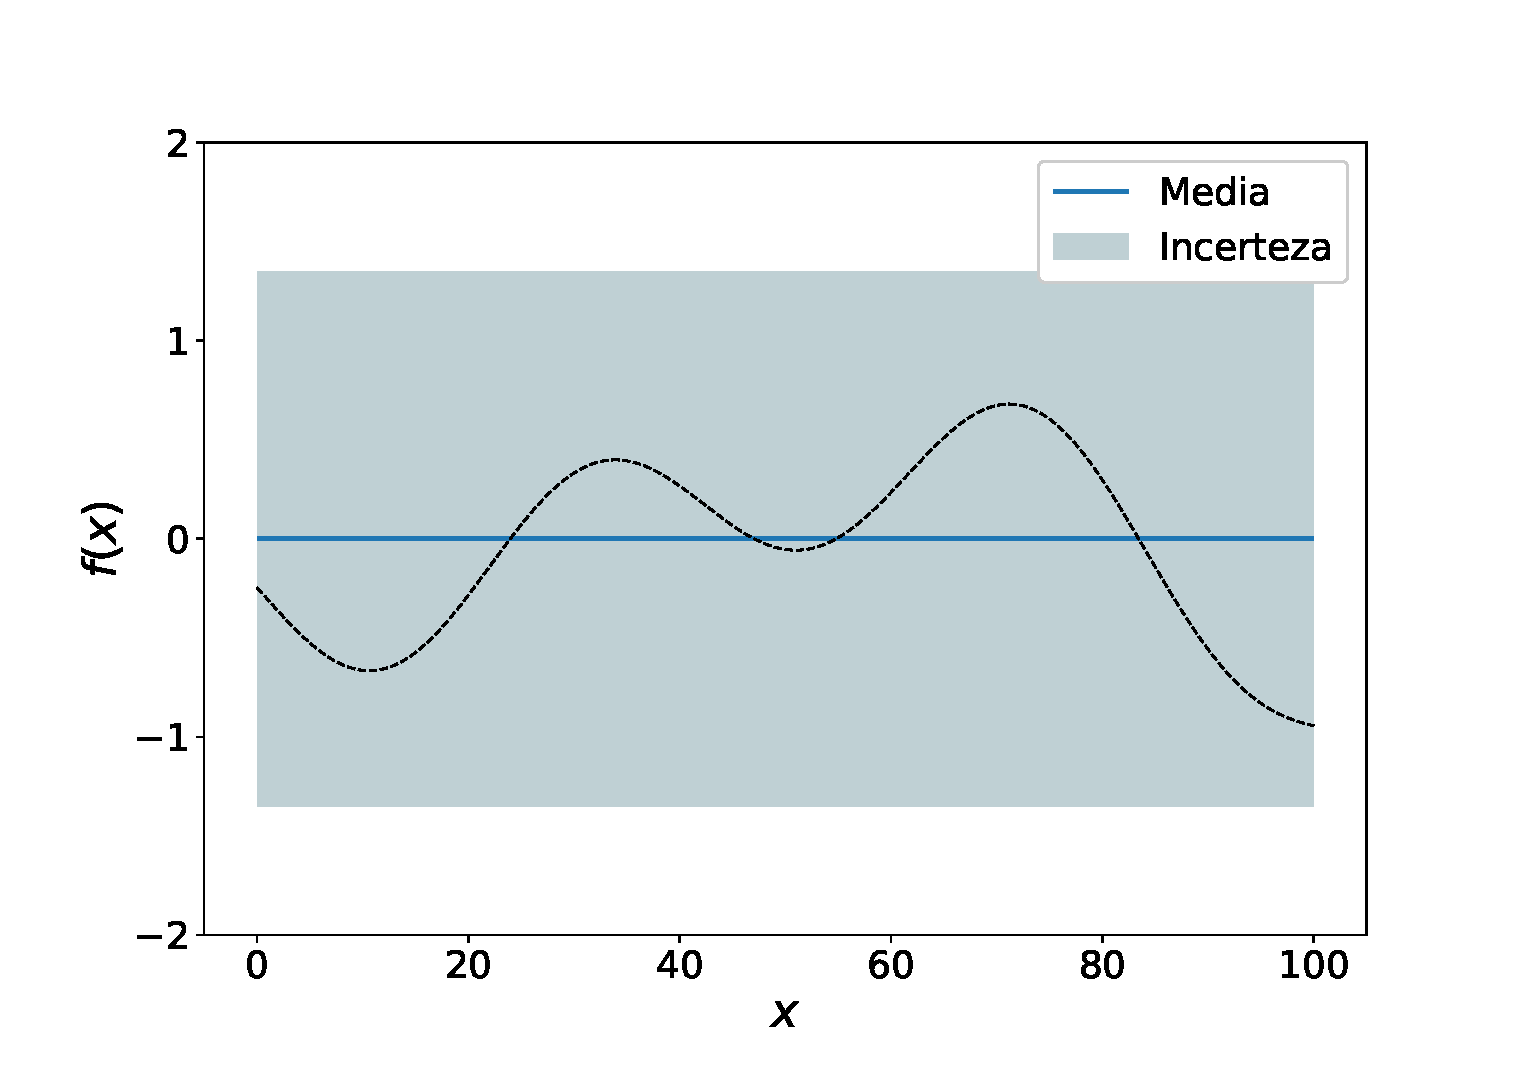
\includegraphics[width=0.31\textwidth]{figures/gp/funcion.eps} 
 \includegraphics[width=0.31\textwidth]{figures/gp/func_acq.eps} 
 \includegraphics[width=0.31\textwidth]{figures/gp/eval1.eps} \\
  \includegraphics[width=0.31\textwidth]{figures/gp/eval2.eps}
  \includegraphics[width=0.31\textwidth]{figures/gp/eval3.eps}
  \includegraphics[width=0.31\textwidth]{figures/gp/eval4.eps} \\
  \includegraphics[width=0.31\textwidth]{figures/gp/eval5.eps}
  \includegraphics[width=0.31\textwidth]{figures/gp/eval6.eps}
  \includegraphics[width=0.31\textwidth]{figures/gp/eval7.eps} 
\end{figure}

\begin{itemize}
\item kernel, 
\item tipo de mapeo, 
\item función de adquisión, 
\item evaluaciones iniciales,
\item costo, 
\item número de evaluaciones.
\end{itemize}

\newpage
%=======================================================================
\section{Resultados}

En esta sección presentamos los resultados obtenidos de la optimización
del átomo de berilio con estado de carga neutral. Los resultados son 
presentados y analizados en las siguientes subsecciones: energía de 
ionización, energías de excitación, fuerzas de oscilar y secciones 
eficaces de excitación por impacto de electrón. En el ajuste del blanco 
aplicamos el método de optimización bayesiana con procesos gaussianos, 
descrito en la Sección~\ref{sec:gaussianprocess}, mediante la 
implementación del código GPyOpt~\cite{GPyOpt}.

Como hemos establecido en este capítulo, la descripción de los blancos 
atómicos está determinado por tres variables:
\begin{itemize}
\item las configuraciones electrónicas incluidas en el CI,
\item los potenciales modelos definidos en la ecuación radial de 
Schr\"odinger, y
\item los parámetros de escala que definen dichos potenciales.
\end{itemize}
En el presente trabajo, estudiamos la optimización de la estructura 
atómica del Be en el proceso de excitación por impacto de electrón 
considerando solo la última de estas variables. Para ello, definimos a 
priori las configuraciones electrónicas y los modelos potenciales que
modelan dicha estructura. Las configuraciones electrónicas incluidas en
en el modelado de Be a lo largo de esta sección fueron $2s^2$, $2snl$ 
tal que $n=1-5$ y $l=0-4$, $2p^2$, y $2pnl$ siendo $n=3-5$ y $l=0-4$, 
donde los orbitales $5l$ se han supuesto pseudo-orbitales. Esto resulta 
en un total de 90 términos, donde sólo 19 de ellos son términos 
espectroscópicos. %el resto se ubica por arriba de la energía de ionización
Por otro lado, los potenciales modelos elegidos fueron aquellos que mejor 
describen, sin ningún tipo de ajuste paramétrico, las energías y fuerzas 
de oscilador. Con este criterio, se determinó implementar el potencial 
STO, más un término de intercambio local, y el potencial de correlación 
core-valencia de Norcross.

La optimización del blanco fue ejecutada en etapas, con el fin de 
comprender en profundidad este proceso. En primera instancia, se 
ajustaron los parámetros que definen el potencial de polarización de 
Norcross. Luego, fijando los parámetros de Norcross resultantes, se 
procedió a ajustar el potencial STO. Para estudiar el efecto de la 
optimización del potencial de Hartree, este procedimiento también fue 
encarado por partes. Cada una de estas partes se corresponde a una capa
definida por el número cuántico principal $n$. Así, al ajuste del 
potencial STO consistió en optimizar los términos de excitación 
correspondientes a los orbitales $3l$, $4l$ y $5l$, de forma sucesiva.

\subsection{Energía de ionización}

La introducción del potencial de polarización de Norcross nos permite
ajustar la energía de ionización del berilio a su valor experimental,
$E_I=0.6852$ Ry~\cite{NIST}. La ecuación \ref{eq:Norcross-pot} está 
compuesta por el conjunto de parámetros $\{\alpha_l,\rho_l\}$, donde 
$l=0,1,2$. Así, se define un espacio de seis hiper-parámetros. El 
parámetro $\alpha$ es la polarizabilidad de core. Así, el espacio de 
búsqueda fue definido alrededor de su valor experimental 
(0.05123~\cite{Dalgarno:62} y 0.05224~\cite{Sitz:71}), y dentro de un 
rango de exploración significativo, dado por
\begin{equation}
\boldsymbol\alpha=[0.0010-0.2000]\,.
\end{equation}
Por otro lado, el parámetro $\rho$ nos da más libertad para ajustar la 
energía de ionización con su valor experimental. Así, el rango de 
exploración para este parámetro fue definido como
\begin{equation}
\boldsymbol\rho=[0.2000-1.5000]\,.
\end{equation}

La función de costo implementada para ajustar el potencial de 
polarización del core fue definida como
\begin{equation}
J_{\mathrm{pol}} = \sum_{i=2}^N \left|\frac{E_{i}-E_{i}^{\textrm{comp.}}
(\boldsymbol{\lambda})}{E_{i}} \right|
\end{equation}
donde $E_{i}$ es la energía absoluta observada (energía de ionización más
energía de excitación) del término $i$--ésimo y $\tilde{E}_{i}}$ es su 
contraparte teórica, la cual depende de los parámetros 
$\boldsymbol{\lambda}$ y de los potenciales modelos elegidos.

El diseño inicial de la optimización incluyó un mapeo tipo latin 
hypercube, un kernel RBF (square exponential) y una función de adquisión 
de EI. El número inicial de evaluaciones fue de \texttt{initer}, con un 
presupuesto de \texttt{maxeval}. 

\newpage
\subsection{Energías de excitación}




\begin{table}
\centering
\begin{tabular}{|cc|ccccc|}
\hline 
No & Término      & NIST & Sin opt. & BO $3l$ & BO $4l$ & BO $\bar{5l}$ \\
\hline 
\hline 
1 & $2s^2\,^1S$   & 0.0000 & 0.0000 & 0.0000 & 0.0000 & 0.0000 \\
2 & $2s2p\,^3P^*$ & 0.2003 & 0.2040 & 0.1996 & 0.1989 & 0.1977 \\
3 & $2s2p\,^1P^*$ & 0.3879 & 0.4225 & 0.4079 & 0.3953 & 0.4007 \\
4 & $2s3s\,^3S$   & 0.4746 & 0.4732 & 0.4749 & 0.4744 & 0.4765 \\
5 & $2s3s\,^1S$   & 0.4983 & 0.5016 & 0.4962 & 0.5005 & 0.5002 \\
6 & $2p^2\,^1D$   & 0.5184 & 0.6598 & 0.5203 & 0.5183 & 0.5165 \\
7 & $2s3p\,^3P^*$ & 0.5368 & 0.5376 & 0.5373 & 0.5353 & 0.5353 \\
8 & $2p^2\,^3P$   & 0.5440 & 0.5595 & 0.5442 & 0.5501 & 0.5466 \\
9 & $2s3p\,^1P^*$ & 0.5485 & 0.5574 & 0.5569 & 0.5478 & 0.5498 \\
10 & $2s3d\,^3D$  & 0.5655 & 0.5665 & 0.5582 & 0.5653 & 0.5642 \\
11 & $2s3d\,^1D$  & 0.5871 & 0.5322 & 0.5874 & 0.5892 & 0.5881 \\
\hline
\multicolumn{2}{l}{Energía de ionización} & 0.6852 & 0.6874 & 0.6774 & 0.6847 & 0.6846  \\ 
\hline
\end{tabular}
\caption[Energías de excitación de Be.]
{Energía en Rydbergs de los primeros 11 términos de Be relativos 
al término fundamental $2s^2\,^1S$.}
\label{tab:exener}
\end{table}

\begin{figure}
\centering
\includegraphics[width=\textwidth]{figures/rmatrix/erp_ei.eps} 
\caption[Error relativo de los primeros 10 términos de excitación.]
{Error relativo de los primeros 10 términos de energía de excitación.}
\label{fig:exener}
\end{figure}

\newpage
\subsection{Fuerzas de oscilador de asborción}

\begin{table}
\begin{adjustwidth}{-.6in}{-.6in}  
\centering
\begin{tabular}{|lllllllll|} 
\hline 
No & Transición               & Ballance   & Chen       & MCHF       & No opt.    & BO $3l$    & BO $4l$  & BO $5l$ \\
\hline
\hline
1 & $2s2  \,^1S - 2s2p \,^1P$ & $1.37$ & $1.38$ & $1.38    $ & $1.32    $ & $1.35    $ & $1.38    $ & $1.31$ \\
2 & $2s2  \,^1S - 2s3p \,^1P$ & $1.12[-2]^\dagger$ & $9.01[-3]$ & $8.99[-3]$ & $5.70[-2]$ & $6.47[-2]$ & $1.12[-2]$ & $2.14[-2]$ \\
3 & $2s2p \,^3P - 2s3s \,^3S$ & $7.56[-2]$ & $8.23[-2]$ & $8.41[-2]$ & $8.57[-2]$ & $1.28[-1]$ & $7.37[-2]$ & $7.27[-2]$ \\
4 & $2s2p \,^3P - 2s3d \,^3D$ & $2.99[-1]$ & $2.95[-1]$ & $3.00[-1]$ & $2.96[-1]$ & $3.94[-1]$ & $2.70[-1]$ & $2.68[-1]$ \\
5 & $2s2p \,^1P - 2s3s \,^1S$ & $1.20[-1]$ & $1.18[-1]$ & $1.15[-1]$ & $1.62[-1]$ & $1.80[-1]$ & $1.14[-1]$ & $1.27[-1]$ \\
6 & $2s2p \,^1P - 2s3d \,^1D$ & $3.86[-1]$ & $4.10[-1]$ & $3.96[-1]$ & $8.18[-2]$ & $2.57[-1]$ & $3.45[-1]$ & $3.36[-1]$ \\
7 & $2s3s \,^3S - 2s3p \,^3P$ & $1.02$     & $1.13    $ & $1.14    $ & $1.15    $ & $9.11[-1]$ & $1.09    $ & $1.026$ \\
8 & $2s3s \,^1S - 2s3p \,^1P$ & $9.08[-1]$ & $9.58[-1]$ & $9.47[-1]$ & $9.02[-1]$ & $7.56[-1]$ & $9.04[-1]$ & $9.16[-1]$ \\
9 & $2s3p \,^3P - 2s3d \,^3D$ & $4.83[-1]$ & $5.01[-1]$ & $5.14[-1]$ & $4.92[-1]$ & $3.27[-1]$ & $5.06[-1]$ & $4.88[-1]$ \\
10 & $2s3p \,^1P - 2s3d \,^1D$ & $6.91[-1]$ & $6.87[-1]$ & $6.81[-1]$ & $9.26[-2]$ & $7.93[-1]$ & $6.96[-1]$ & $6.67[-1]$ \\
\hline
\multicolumn{2}{c}{$\dagger\,a[b]$ denotes $a\times 10^b$} \\
\end{tabular}
\caption{Fuerza de oscilador de absorción de Be.}
\label{tab:fabs}
\end{adjustwidth}
\end{table}


\begin{figure}
\centering
\includegraphics[width=\textwidth]{figures/rmatrix/fabs.eps} 
\caption{Fuerza de oscilador de absorción del Be.}
\label{fig:fabs}
\end{figure}

\newpage
\subsection{Excitación por impacto de electrón}


\begin{figure}
\centering
\includegraphics[width=\textwidth]{figures/rmatrix/opt_nl.eps} 
\caption[Secciones eficaces de excitación por impacto de electrón en Be.]
{Secciones eficaces de excitación por impacto de electrón en Be.
Curvas: Dipti \textit{et al.}~\cite{Dipti:19} (discontinua), RMPS sin 
ajuste (punteada); cálculos con optimización bayesiana: 
$3l$ (raya-punto), 
$4l$ (raya-punto-punto), y
$5l$ (continua). 
Símbolos: cálculos CCC de \cite{Fursa:97}.}
\end{figure}

\newpage
%=======================================================================
\section{Conclusiones}
